% ============================================================
%  IEEE Transactions on Emerging Topics in Computing
%  Implementation Paper Draft
%  Title: Let It Compile: An RL Approach to Adaptive Register Allocation for GPU Kernel Optimization Across the Stack
%  Authors: Sanchitsai Nipanikar, Sandip Shinde, Sangita Lade, VIT Pune
% ============================================================

\documentclass[journal,letterpaper]{IEEEtran}

% --------------- Packages ---------------
\usepackage{amsmath,amsfonts,amssymb}
\usepackage{array}
\usepackage[caption=false,font=normalsize,labelfont=sf,textfont=sf]{subfig}
\usepackage{textcomp}
\usepackage{stfloats}
\usepackage{url}
\usepackage{graphicx}
\usepackage{booktabs}
\usepackage{multirow}
\usepackage{cite}
\usepackage{balance}
\usepackage{tikz}
\usetikzlibrary{shapes.geometric, arrows.meta, positioning, fit, backgrounds, calc}

\hyphenation{op-tical net-works semi-conduc-tor IEEE-Xplore Num-ba Gym-na-sium}

% ============================================================
\begin{document}
% ============================================================

\title{Let It Compile: An RL Approach to Adaptive Register Allocation\\for GPU Kernel Optimization Across the Stack}

\author{Sanchitsai~Nipanikar,~Sandip~Shinde,~Sangita~Lade%
\thanks{S.~Nipanikar is with the Department of Computer Engineering,
Vishwakarma Institute of Technology, Pune~411037, Maharashtra, India.
E-mail: sanchitsai.nipanikar22@vit.edu}%
\thanks{S.~Shinde is with the Department of Computer Engineering,
Vishwakarma Institute of Technology, Pune~411037, Maharashtra, India.
E-mail: sandeep.shinde@vit.edu}%
\thanks{S.~Lade: affiliation and e-mail to be added.}%
\thanks{Manuscript received \today.}}

\markboth{IEEE Transactions on Emerging Topics in Computing,~Vol.~XX,
No.~X, 2026}%
{Nipanikar \MakeLowercase{\textit{et al.}}: Let It Compile}

\maketitle

% ============================================================
%  ABSTRACT
% ============================================================
\begin{abstract}
Just-in-time (JIT) compilation is a practical route to accelerating Python GPU workloads, but performance depends on low-level launch and compilation choices whose optimal settings vary across kernels, input sizes, and driver constraints.
This paper presents an implementation of a reinforcement learning (RL) loop that learns to tune two JIT-exposed GPU knobs---thread-block size and per-thread register cap---for Numba CUDA kernels.
The system is implemented as a Gymnasium environment~\cite{gymnasium} with stable-baselines3~\cite{sb3} PPO~\cite{ppo2017} and supports two measurement backends: (i) a low-overhead NVML telemetry path~\cite{nvml} for fast training and (ii) a CUPTI-derived counter path collected via Nsight Compute CLI~\cite{nsightcompute,cupti} for targeted analysis.

On an NVIDIA GeForce RTX 3050 Laptop GPU (Windows/WDDM), NVML-only PPO training for 50{,}000 steps completes in 590 seconds (84.7 steps/s).
In evaluation over three kernels (GEMM, reduction, softmax) and three problem sizes ($N\in\{256,512,1024\}$), the learned policy achieves up to $3.02\times$ speedup over a per-episode baseline configuration, with the strongest mean improvements observed for softmax ($1.92\times$ at $N{=}512$; $1.74\times$ at $N{=}1024$).
We also document failure modes encountered when profiling per step with Nsight Compute on Windows, motivating a hybrid workflow: train with NVML signals and reserve CUPTI counters for short rollouts.
\end{abstract}

\begin{IEEEkeywords}
GPU kernels, JIT compilation, Numba, reinforcement learning, PPO, autotuning, register capping, NVML, Nsight Compute, Windows.
\end{IEEEkeywords}

% ============================================================
%  I. INTRODUCTION
% ============================================================
\section{Introduction}
\label{sec:intro}

\IEEEPARstart{P}{ython}-first GPU programming has become common in machine learning and scientific computing.
Frameworks and JIT systems make it easy to write CUDA kernels in high-level languages, but they also expose a multi-layer performance problem: the effective runtime of a kernel is shaped jointly by the source program, the JIT compiler, the GPU launch configuration, and resource allocation decisions such as register usage.

This project targets a concrete, implementation-driven question: \emph{can an RL agent learn to tune JIT-time GPU knobs using only signals that are practical to collect on Windows?}
Windows adds a key constraint: fine-grained hardware counter collection (CUPTI) is often slow or permission-gated under WDDM, while lightweight telemetry (NVML) is accessible but coarse.

\subsection{Contributions}
This paper makes the following contributions:
\begin{itemize}
\item An end-to-end, reproducible implementation of RL-guided JIT tuning for Numba CUDA kernels using a Gymnasium environment and PPO.
\item A measurement pipeline that supports both NVML-only training (fast) and CUPTI-derived counters via Nsight Compute CLI (accurate but expensive).
\item An experimental evaluation on three representative kernels and three sizes, including a results table derived from saved CSV artifacts.
\item A practical characterization of Windows profiling overhead and stability issues that arise when profiling each environment step.
\end{itemize}

% ============================================================
%  II. BACKGROUND
% ============================================================
\section{Background and Motivation}
\label{sec:background}

Numba~\cite{numba2015} compiles Python functions decorated with \texttt{@cuda.jit} into GPU kernels at runtime, enabling rapid iteration while still generating PTX and SASS via the CUDA toolchain.
However, JIT compilation does not eliminate tuning: launch geometry and compilation options can significantly shift occupancy, memory behavior, and total runtime.

We focus on two JIT-time knobs that are (a) exposed in a simple way in Numba and (b) impactful for occupancy/performance trade-offs:
\begin{enumerate}
\item \textbf{Thread-block size} (discrete choices), influencing scheduling and memory coalescing.
\item \textbf{Register cap} (\texttt{max\_registers}), acting like \texttt{ptxas --maxrregcount} and trading per-thread registers for occupancy.
\end{enumerate}

The challenge is that the best combination depends on kernel structure and input size.
Hand-tuned heuristics exist but do not adapt online.
We therefore model tuning as sequential decision-making.

% ============================================================
%  III. SYSTEM OVERVIEW
% ============================================================
\section{System Overview}
\label{sec:system}

Fig.~\ref{fig:system} shows the implemented loop.
At each step, the policy selects a discrete action $(b, r)$ that chooses a block size $b$ and a register cap $r$.
The environment compiles (or reuses a cached compile of) the corresponding Numba kernel, runs a short microbenchmark, collects telemetry/counters, and returns an observation and reward.

\begin{figure}[t]
\centering
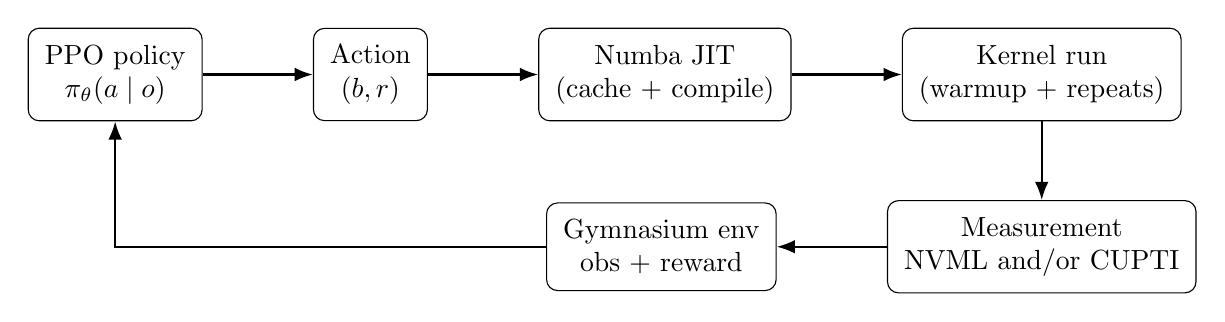
\begin{tikzpicture}[
  node distance=7mm,
  box/.style={rectangle, rounded corners, draw, align=center, inner sep=6pt},
  arrow/.style={-Latex, thick}
]

\node[box] (policy) {PPO policy\\$\pi_\theta(a\mid o)$};
\node[box, right=14mm of policy] (action) {Action\\$(b, r)$};
\node[box, right=14mm of action] (jit) {Numba JIT\\(cache + compile)};
\node[box, right=14mm of jit] (run) {Kernel run\\(warmup + repeats)};
\node[box, below=10mm of run] (measure) {Measurement\\NVML and/or CUPTI};
\node[box, left=14mm of measure] (env) {Gymnasium env\\obs + reward};

\draw[arrow] (policy) -- (action);
\draw[arrow] (action) -- (jit);
\draw[arrow] (jit) -- (run);
\draw[arrow] (run) -- (measure);
\draw[arrow] (measure) -- (env);
\draw[arrow] (env) -| (policy);

\end{tikzpicture}
\caption{End-to-end RL-guided JIT tuning loop implemented in this work.}
\label{fig:system}
\end{figure}

% ============================================================
%  IV. RL FORMULATION
% ============================================================
\section{Reinforcement Learning Formulation}
\label{sec:rl}

We cast kernel tuning as a Markov decision process (MDP) with episode-specific baselines.
An episode fixes a kernel $k$ and size $N$ and runs for a maximum number of steps.

\subsection{Action space}
The action is a pair $(b, r)$ drawn from a small discrete set:
\begin{equation}
  b \in \{64, 128, 256\},\quad r \in \{0, 32, 64\},
\end{equation}
where $r{=}0$ indicates ``no cap'' (compiler default).

\begin{table}[t]
\centering
\caption{Discrete tuning knobs (action space).}
\label{tab:action_space}
\begin{tabular}{ll}
\toprule
Knob & Values \\
\midrule
Block size $b$ & 64, 128, 256 \\
Register cap $r$ & 0 (default), 32, 64 \\
\bottomrule
\end{tabular}
\end{table}

\subsection{Observation space}
Observations are normalized to $[0,1]$ and include (i) a small vector of CUPTI-derived metrics when enabled, (ii) a 4D NVML telemetry vector (utilization, memory utilization, memory used, temperature), (iii) a one-hot kernel identifier, and (iv) the previous action indices.
When CUPTI is disabled or unavailable, its portion of the observation is zero.

\subsection{Reward}
Each episode computes a baseline time $t_{\text{base}}$ using a fixed reference action (block size 256, default registers).
After executing an action at time $t$, we compute speedup and reward as:
\begin{align}
  \text{speedup} &= \frac{t_{\text{base}}}{t},\\
  r &= \text{speedup} - 1.
\end{align}
This keeps the baseline near zero reward and makes improvements positive.

% ============================================================
%  V. IMPLEMENTATION
% ============================================================
\section{Implementation Details}
\label{sec:impl}

\subsection{Kernels and JIT knobs}
We implement three Numba CUDA kernels: tiled GEMM, a reduction, and a row-wise softmax.
The register-cap knob is implemented using Numba's \texttt{cuda.jit(max\_registers=\dots)} wrapper, which re-JITs a Python kernel function with a per-thread register limit.
Kernel variants are cached to avoid recompiling the same configuration repeatedly.

\subsection{Timing}
Kernel timing uses CUDA events to measure mean runtime across a small number of repeats, with a warmup to trigger compilation.
The environment includes defensive handling for rare CUDA context degradation events on long profiler-heavy runs.

\subsection{Telemetry (NVML)}
NVML~\cite{nvml} is used as a low-overhead source of GPU utilization and memory signals.
On Windows, utilization is reported on a coarse sampling window; when a step is long enough (e.g., when a profiler subprocess runs), polling NVML concurrently yields more stable peak-utilization features.

\subsection{Hardware counters (CUPTI via Nsight Compute)}
For detailed analysis, we collect a small, stable set of metrics by invoking Nsight Compute (\texttt{ncu})~\cite{nsightcompute} as a subprocess and parsing its CSV output.
This avoids directly binding to the CUPTI C API on Windows, but it introduces large per-step overhead and may fail without Administrator permissions (e.g., \texttt{ERR\_NVGPUCTRPERM}).

% ============================================================
%  VI. EXPERIMENTAL SETUP
% ============================================================
\section{Experimental Setup}
\label{sec:setup}

\subsection{Platform}
Experiments were run on Windows with an NVIDIA GeForce RTX 3050 Laptop GPU (4.29~GB).

\subsection{Training configuration}
We train PPO for 50{,}000 steps with NVML enabled and CUPTI disabled.
The saved training configuration uses batch size 1024, learning rate $3\times10^{-4}$, $\gamma{=}0.99$, GAE $\lambda{=}0.95$, clip range 0.2, entropy coefficient 0.01, and maximum episode length 40.
The training run completed in 590 seconds (9.83 minutes), corresponding to 84.7 environment steps per second.

\subsection{Evaluation protocol}
We evaluate the learned policy using rollout logging: for each kernel and $N\in\{256,512,1024\}$ we run 5 episodes and record an episode summary including the per-episode baseline and the best achieved speedup within the episode.
All reported numbers in Sec.~\ref{sec:results} are computed from the saved CSV artifact.

% ============================================================
%  VII. RESULTS
% ============================================================
\section{Results}
\label{sec:results}

Table~\ref{tab:episode_results} summarizes the evaluation.
For each kernel and size, we report the mean baseline runtime (in milliseconds) and the distribution of best speedup values achieved within an episode.

\begin{table}[t]
\centering
\caption{Evaluation summary from the episode-level CSV artifact (5 episodes per case). ``Best speedup'' is relative to the per-episode baseline.}
\label{tab:episode_results}
\begin{tabular}{llrrl}
\toprule
Kernel & $N$ & Baseline mean (ms) & Best speedup mean & Best speedup range \\
\midrule
GEMM & 256 & 0.212 & 1.22 & [1.06, 1.60] \\
GEMM & 512 & 0.865 & 1.03 & [0.98, 1.11] \\
GEMM & 1024 & 5.309 & 1.04 & [1.00, 1.15] \\
Reduction & 256 & 0.102 & 1.52 & [1.04, 2.90] \\
Reduction & 512 & 0.094 & 1.03 & [0.99, 1.09] \\
Reduction & 1024 & 0.292 & 1.03 & [0.68, 1.16] \\
Softmax & 256 & 0.389 & 1.26 & [1.13, 1.46] \\
Softmax & 512 & 1.170 & 1.92 & [1.40, 2.21] \\
Softmax & 1024 & 2.405 & 1.74 & [1.41, 3.02] \\
\bottomrule
\end{tabular}
\end{table}

\subsection{Key observations}
\begin{itemize}
\item \textbf{Softmax benefits most from tuning.} At $N{=}512$ the mean best speedup is $1.92\times$, and at $N{=}1024$ the maximum best speedup reaches $3.02\times$.
\item \textbf{Reduction shows high variance at small sizes.} At $N{=}256$ the best speedup range spans $1.04\times$ to $2.90\times$, consistent with sensitivity to launch configuration and measurement noise at very short runtimes.
\item \textbf{GEMM improvements are modest at larger sizes.} The mean best speedup for GEMM is near $1.03\times$--$1.04\times$ for $N\ge512$ in this evaluation.
\end{itemize}

% ============================================================
%  VIII. DISCUSSION AND LIMITATIONS
% ============================================================
\section{Discussion and Limitations}
\label{sec:limits}

\subsection{Why NVML-first on Windows}
Collecting CUPTI-derived counters with Nsight Compute provides richer state, but invoking \texttt{ncu} per environment step can take seconds per step and may destabilize the CUDA context after long runs.
In contrast, NVML signals have low overhead and enabled a complete 50k-step PPO run in under 10 minutes.

\subsection{Measurement variability}
Short kernels are sensitive to both JIT warmup effects and OS-level scheduling.
We mitigate this with warmup and repeated timing, but residual noise remains, especially for very small runtimes.

\subsection{Scope}
The current action space is intentionally small (3 block sizes and 3 register caps) to keep training stable and to match Phase-0/1 exploration.
Extending to larger discrete sets, continuous knobs, or multi-kernel scheduling is future work.

% ============================================================
%  IX. CONCLUSION
% ============================================================
\section{Conclusion}
\label{sec:conclusion}

This paper presented an implementation of an RL loop for adaptive register capping and launch-configuration tuning for Python GPU kernels.
Using a practical NVML-only training path on Windows, PPO learns tuning policies that deliver consistent speedups for softmax and selective gains on reduction and GEMM.
The implementation also highlights a pragmatic hybrid workflow for Windows: train with low-overhead telemetry and reserve hardware counter collection for short, research-grade rollouts.

\balance

\section*{Acknowledgment}
The authors thank the Department of Computer Engineering at Vishwakarma Institute of Technology, Pune, for research infrastructure and support.

% ============================================================
%  REFERENCES
% ============================================================
\begin{thebibliography}{10}

\bibitem{numba2015}
S.~K.~Lam, A.~Pitrou, and S.~Seibert, ``Numba: A LLVM-based Python JIT compiler,'' in \textit{Proc.\ 14th Python in Science Conf.\ (SciPy)}, 2015.

\bibitem{ppo2017}
J.~Schulman, F.~Wolski, P.~Dhariwal, A.~Radford, and O.~Klimov, ``Proximal Policy Optimization Algorithms,'' \textit{arXiv:1707.06347}, 2017.

\bibitem{sb3}
A.~Raffin, A.~Hill, A.~Gleave, A.~K. Kanervisto, M.~Ernestus, and N.~Dormann, ``Stable-Baselines3: Reliable Reinforcement Learning Implementations,'' \textit{J. Mach. Learn. Res.}, vol.~22, no.~268, pp.~1--8, 2021.

\bibitem{gymnasium}
Farama Foundation, ``Gymnasium,'' 2023. [Online]. Available: \url{https://gymnasium.farama.org/}

\bibitem{nvml}
NVIDIA Corporation, ``NVIDIA Management Library (NVML),'' 2026. [Online]. Available: \url{https://developer.nvidia.com/nvidia-management-library-nvml}

\bibitem{nsightcompute}
NVIDIA Corporation, ``Nsight Compute,'' 2026. [Online]. Available: \url{https://developer.nvidia.com/nsight-compute}

\bibitem{cupti}
NVIDIA Corporation, ``CUDA Profiling Tools Interface (CUPTI),'' 2026. [Online]. Available: \url{https://developer.nvidia.com/cupti}

\end{thebibliography}

\end{document}
